\documentclass[11pt]{article}
\usepackage[left=1in, right=1in, bottom=0.5in, top=0.5in]{geometry}
\usepackage{graphicx}
\begin{document}
	
\section*{Response to the Referees}

To whom it may concern,

First we would like to thank the reviewer for their comments, which have helped us improve this manuscript. The paper has now been re-written to fit the Nature format, and therefore some of the content has changed or moved. The main body of the paper is mostly new or adapted writing, and the \textbf{Methods} and \textbf{Supplementary Information} contains details on data, methods, and discussion. At the end of this document we’ve listed any major changes made.

Our responses are below. We’d like to address the bias comment first, as it is the most significant one, and shows up a couple of times in the reviewer’s report. \\

\noindent \textbf{With photometry, rotation is much easier to measure for the stars that are active and faster rotating. Is there a similar bias in the case of seismology? }

In short, yes, there are biases at play, but these do not affect our results. We’ve discussed them below, and have included a version of this discussion in the \textbf{Methods} section of the new draft.

\textit{Bias in rotation detection:} stars that are rotating very slowly will show very small splittings, which may be indistinguishable from a non-rotating case, whereas stars that are spinning very fast may find that their splitting is so wide that they cross over with split modes at different radial orders. We’ve done some calculations to show that this shouldn’t affect the region of rotation we’re interested in.
\begin{enumerate}
\item \textit{Fast rotating stars}: in principle, a star could rotate fast enough that the highest-frequency peak in a split dipole ($\ell=2$) mode would overlap with the radial ($\ell=0$) mode. This would occur if $2\nu_{\rm{s}} > \delta\nu_{02}$. For the star in our sample with the smallest $\delta\nu_{02}$ (so the highest risk of this happening), this limit is at 8.8 days. However for the star with the largest $\delta\nu_{02}$, this lies at ~2 days. 

In practice, the mode frequency model would properly fit a spectrum where this kind of mode-overlapping was happening. The $\ell=0$ modes don’t split, and so if a $\ell=2$ mode were split so far that overlap was occurring, the power distribution of the $\ell=0$ mode would change, which is not degenerate with any other model states. There would also still be a constraint on the splitting from the lower-frequency split components of the $\ell=2$ mode, as well as constraints on the exact mode frequencies and linewidths from fits to other modes in the spectrum. We can envision there being an issue if an $\ell=2$ mode is overlapping with an $\ell=1$ mode at lower frequencies as well, however this would only occur at a rotation rate of 2 days or faster for the star with the smallest $\delta\nu_{01}$.
 
In our sample, there are 9 stars for which we measured splittings greater than the limit of $2\nu_s > \delta\nu{02}$. All these stars showed good agreement with previous work, and were well converged, which implies that asteroseismic models such as ours can handle such mode overlap. As far as our conclusions are concerned, all 9 are either Hot or Subgiant stars, which we show don’t impact our conclusions either way in the paper.

\item \textit{Slow rotating stars:} Below, the reviewer raises concerns that for a limit of $\nu_s < 2\Gamma$ (when the splitting is smaller than the double the linewidth), splitting may not be accurately constrained. This is not the fundamental limit on this measurement, and is instead a soft limit (making detection more difficult in stars low-signal-to-noise). Asteroseismic splitting causes a change in the power distribution in frequency of the modes. Detection of this change makes it possible to measure seismic rotation even when the split components are not fully separated.  It is also worth noting that the non-split radial ($\ell=0$) modes provide strong constraints on the variation of linewidth with frequency. 

 If there is to be a hard limit at which the the effects of splitting can not be measured, we suggest that it is where $\nu_s < 2/T$, two times the frequency bin width. The bin width is set by observing time, so to make an conservative estimate, we can take our star with the shortest observing time  (0.49 years). For this star, the limit on measuring rotation would be ~89 days (and increasing for longer observing baselines). As discussed below, as you get to slower rotation rates it becomes harder to constrain the small rate of mode splitting and so the uncertainty will increase. This is dealt with appropriately in our model comparison through the use of hierarchical models.
\end{enumerate}

Hopefully with this discussion we’ve shown that both the slow (hard limit) and fast (soft limit) limits on measuring rotation with asteroseismology do not affect the analysis driving our conclusions, which is done by stars between 10 and 40 days. We’ve added a plot below which should help illustrate our arguments. The circles represent stars in our sample, coloured by their seismic rotation.\\

\begin{figure}[h!]
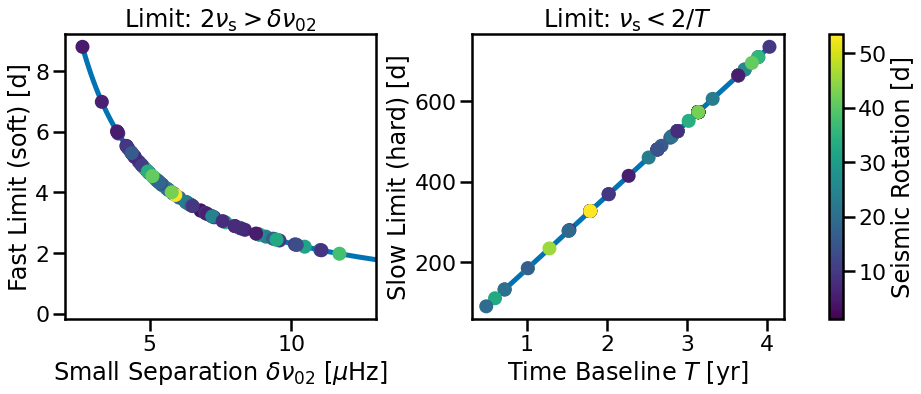
\includegraphics[width=\textwidth]{image1.png}
\caption{Representation of the limits on fast and slow rotation rates. The blue line represents how this limit changes with the small separation (for the fast limit) and the observation baseline (slow limit). The circles represent where stars in our sample fall on these diagrams, and are coloured by their rotation rate.}
\end{figure}

\textit{Bias in stellar populations:} The reviewer/reader might be concerned there is a second potential observational bias in that asteroseismology does not detect stars in the 6200-5800 Kelvin range in the latter half of their main sequence lifetime, and is therefore only detecting younger, faster rotators. This concern is more easily alleviated. The probability of an asteroseismic detection scales with temperature and radius (i.e. scales inversely with log g, and therefore age on the main sequence). More active, magnetic stars may also suppress their oscillation modes, meaning that it is more likely to detect seismic oscillations in older stars.  Because of both these effects asteroseismic detection probabilities are slightly biased towards older stars on the main sequence, not younger. See e.g. Chaplin et al. (2011), Schofield et al. (2019) for Kepler and TESS respectively, and Mathur et al. 2019 for the magnetic suppression.

Between these two statements -- that our method measures accurate rotation in the regions that matter, and that asteroseismology is biased towards older, not younger, stars -- we don’t believe that observing biases affect our conclusions. We’ve included a paraphrased version of the discussion as above in the paper \textbf{Methods} Section 3.4. \\

\noindent\textbf{The significance of the results, would be much stronger if:
\begin{itemize}
\item it could be shown that there is no observational bias
associated with the seismic data and 
\item if a range of rotation evolution models were considered, not just one model with and without weakened breaking.
\end{itemize}
}
With regards to the observational bias, see above.

With regards to the rotation models: It is our opinion that performing this comparison in a separate work would be more appropriate. Most rotation models without weakened magnetic braking will have similar predictions in this regime our sample occupies, as they are all calibrated to reproduce the Sun (and at younger ages, clusters), and so the largest difference between models will come from the inclusion of a change in the braking law. It’s not that we think that such a comparison isn’t important -- on the contrary -- but it should be explored in a separate paper with more of a focus on the differences in theoretical models, and including a much broader range of models both with- and without changes to the braking.\\

\noindent\textbf{One may fear that seismology works only for $\nu_s / \Gamma$ large (ratio of rotational splitting to mode line width, not provided). 
\begin{itemize}
\item How many stars have $\nu_s /  \Gamma < 2$ here (the problematic cases)?
\item How many of these are slow rotators? 
\end{itemize}
}

That seismic rotation can only be probed in cases where split components are fully separated from one another, as the reviewer is suggesting, is a common misconception. Asteroseismic splitting is rarely larger than double the linewidth (in our sample this is only the case for a handful of the fastest rotators). Instead, rotational splitting changes the distribution of a mode's power with frequency, in a way that can be disentangled. This takes a specific form depending on the angular degree of the mode and the inclination angle of the star. This is why marginalising over inclination angle is important, because only by constructing a model that accounts for inclination angle and rotation together can you accurately represent how rotation affects the modes.

It is also worth noting that our fitting method marginalises over inclination angle, rotational splitting and linewidth, and so the final rotational period measurements have uncertainties that accurately reflect the uncertainty associated with the slow rotation only having a small effect on the power distribution of the modes of oscillation. To be clear, there is no boundary beyond which this methodology of measuring asteroseismic rotation no longer works, until you start pushing up against the frequency resolution of the power spectrum (as discussed above).

As discussed at the top of this response, the reviewer may be concerned that Figure 3 (Figure 5 in the old draft) shows  a number of slow rotators that were not included in the model comparison, because they had poor convergence metrics. It is indeed harder to measure rotation in slow rotators (as mentioned above), and so fewer of these stars were able to converge within the computational time we had available. When we repeated the model comparison analysis while still including these stars, our conclusions did not change, a statement which we have now included in the paper.\\

\noindent\textbf{Does the seismic catalog contain enough accurate measurements for the slow rotating stars?}

We are confident that the accuracy of the measurements for the slow rotating stars is sufficient, in this case referring to those with periods of roughly 20 days and up. \textbf{Extended Data} Figures 3 and 4 (Figures 7 and 8 in the old draft) show that stars in this regime are consistent with with previous measurements of asteroseismic rotation where those are available.\\

\noindent\textbf{Is the apparent deficit of slow rotators in the catalog due to weakened magnetic braking or to observational biases? Figure 9 [\textbf{Extended Data} Figure 5 in the new draft] left is not reassuring.}

As discussed above, we believe there is sufficient ground to claim that our deficit of slow rotators is due to weakened magnetic braking and not observational biases in seismology. With regards to \textbf{Extended Data} Figure 5 (Figure 9 in the old draft), as discussed in the text, the disagreements below $5\,  \rm{kms}^{-1}$ are within the expected deviation between seismic and spectroscopic comparisons in this region (Tayar et al. 2015). We’ve added a line to indicate the border of this region. In addition, the majority of slowly rotating stars in the Figure lie above the 1:1 line, implying that if spectroscopic values were the truth, seismology would find rotation rates that are *slower* than the truth, which would bias our results towards a standard model, and not towards weakened magnetic braking.

The spectroscopy comparison is there for completeness, but in our opinion the more important test is the comparison to surface rotation rates (Figure 2 in the new draft), which shows good agreement. A paraphrased version of this answer is now included in the text in \textbf{Methods} Section 3.3.\\

\noindent \textbf{The stellar inclination angle i is clearly not measured, as shown in figure 6-middle [\textbf{Extended Data} Figure 2 in the new draft]. Therefore the stellar rotation rate itself is not determined for individual stars. Is this not a problem for the interpretation of the data in terms of rotation evolution models, esp. toward the slow-rotator end of the distribution?}

The purpose of \textbf{Extended Data} Figure 2 (Figure 6 in the old draft) is to check whether our inclination angle returns the prior. In the majority of cases the spread of the posterior distribution is smaller than the prior, indicating that our measurement of $i$ is driven by the data. Even in the cases where it does closely resemble the prior, our Bayesian approach will ensure that this is properly reflected in the results for the rotation period. In our analysis, rotational splitting ($\nu_{s}\sin(i)$), inclination ($i$) and rotation ($P$) are all marginalised over, and so the uncertainties reflect the posterior probability distribution these values can take given the data. Because of this, the uncertainties on rotation visible in the Figure have already accurately incorporated the uncertainty in the inclination angle. We have added extra description to the figure caption that clarifies this. The stellar rotation rate is well determined for individual stars in spite of the difficulties with constraining inclination angle, because it has been fully marginalised over in our Bayesian analysis.

If I’m interpreting the reviewer’s report correctly, we understand that they are concerned that there are fewer slowly rotating stars, and that those that are slowly rotating appear to have large uncertainties. There are relatively few stars in this slowly rotating regime, and we address this in the comments about observational bias above. We don’t think the larger uncertainties should raise concern. The latent variable model we use to compare the two rotational evolution models allowed us to incorporate the uncertainties appropriately, and bear in mind that it’s not just rotation space where the models are compared, but mass, metallicity, temperature, and age as well.\\

\noindent\textbf{ Two rotation evolution models are tested against each other. One model is favoured (more likely than the other). However, it is not clear how good is this model, i.e. whether it fits the data. In particular, it is not clear whether the data really favour a transition model and not another spin-down model (e.g., Matt et al. 2015).}

Our model is based on the Matt formalism, although our choices of scalings for stellar angular momentum loss and magnetism are different (see van Saders et al. 2019), and so our models are more similar to the Matt models than other models available in the literature (see Fig 1 in Matt et al. 2015) 

The Matt et al. 2015 model and associated paper puzzled over the fact that the apparent edge of the period distribution in the McQuillan sample was at roughly the solar age in their model (see fig 3 in Matt 2015), and wondered whether it meant the age distribution in the Kepler field was very different (younger) than expected. Their 4 Gyr model is already at the McQuillan period distribution edge. Their model would have predicted the same long rotation periods as our standard model, with differences in detail because of the different braking law scalings. In other words: a 8-9 Gyr star in the Matt model would not be sitting on that McQuillan edge, it would be above it.

Of course, there are still other models of rotational evolution worth comparing to. Comparing our seismic rotation sample to different models (both with- and without magnetic braking present) is an important next step for this research, but not one we feel belongs in this paper. With this study, we’re really focused on repeating the research that first proposed weakened magnetic braking (van Saders et al. 2016) with the improved seismic sample that includes rotation.\\

\noindent\textbf{The authors may consider making a plot like Figure 2 from van Saders et al. 2016, i.e. ratio of $P_{\rm obs}/P_{\rm predicted}$ versus age. The advantage for plotting the ratio is that it is easier to see whether there is a transition in the data (less impact from the systematic biases in the models).}

We considered including such a plot in our paper, but omitted it because such a plot would not provide any new information beyond what is already included in the paper. The core of this paper is the use of a probabilistic analysis of a full ensemble of stars to distinguish between two competing models. A plot that shows that \textit{individual} stars are in \textit{disagreement} with a standard evolution doesn’t add any new information, especially when the format requires conciseness (and the discrepancy already been demonstrated in previous work for many stars in this sample). We think it is more important to tread new ground with a Bayesian method that accounts for multiple parameter spaces (metallicity being the most important one), to drive our conclusions.

A $P_{\rm obs}/P_{\rm predicted}$  plot would also require us to either model the rotation of individual stars, or delve into empirical gyrochronology, both of which are outside the scope of this paper in its current form, and are better explored in separate work.\\

\noindent\textbf{ Does TRILEGAL correctly synthesize the stellar population? Any free parameters?}

To the best of our knowledge the TRILEGAL simulation is appropriate for this purpose, and any issues that may arise through the use of TRILEGAL are also mitigated by our treatment in the paper--- drawing from TRILEGAL simulated stars until they match the distributions seen by Berger et al. (2020) in the Kepler field. As for the parameters, our TRILEGAL simulation is the same as that used for van Saders et al. (2019), and is using the standard values from Girardi et al. (2005), as described in both those papers (this was wrongly cited as Girardi et al. 2015 in the first draft, and has since been corrected). \\

\noindent\textbf{ Should the paper be published, I would suggest to move most of the asteroseismology details to an appendix at the end of the paper (the asteroseismic analysis is mostly standard). Even though these details are important, the reader should not be diverted from the main topic of the paper, ie the discussion about the rotation evolution models.
Some sections, for example 3.1.4, contain a lot of jargon and are hard to follow even for a specialist. }

There’s been quite a bit of a reshuffle between drafts here to match the Nature Astronomy style. Section 3.1 (the asteroseismic methods) is now in \textbf{Supplementary Information}, which has improved the flow a lot. The Gyrochronology methods and the majority of the discussion are now in \textbf{Methods}, so the core body of the paper is a lot more streamlined.

When transferring the methods to the Supplementary Information, we have tried to improve the explanations of the more complicated terms (such as Gaussian Processes), and have hopefully improved this somewhat.

\clearpage
\section*{Changes to the manuscript}
\subsection*{Structural Changes}
There has been a major structural overhaul of the manuscript to help it comply with the Nature Astronomy guidelines.

\begin{itemize}
	\item The detailed sections of Section 2: Data have been moved to \textbf{Methods}.
	\item Section 3.1: Asteroseismic Model has been moved to \textbf{Supplementary Data}.
	\item Section 3.2: Distinguishing between Gyrochronology Models has been moved to \textbf{Methods}
	\item Portions of the \textit{Fitting Procedure} components of both Model sections are now included in the \textbf{Methods} section.
	\item The detailed sections of Section 4: Results have been moved to \textbf{Methods}.
	\item Table 1 is has been moved to \textbf{Extended Data}.
	\item Section 5.1.1., 5.1.2., and the spectroscopy half of 5.1.3. have all been moved to \textbf{Methods}. Their conclusions are mentioned in the main text.
	\item Section 5.2.2, 5.2.3. and 5.2.4. have all been moved to \textbf{Methods.} Their conclusions are mentioned in the main text.
	\item Figures 3, 6, 7, 8 and 9 have been moved to \textbf{Extended Data} and are referenced from \textbf{Methods}.
	\item Figure 2 has been moved to \textbf{Supplementary Information}.
\end{itemize}

\subsection*{Content Changes}
The main body of the text (pages 2 through 10) is either new or paraphrased from sections of the previous manuscript. We have tried to retain the same contents and citations as in the previous manuscript, to avoid the need for in-depth review of this section of the paper.

Other changes include:
\begin{itemize}
	\item Figure captions have been updated with extra descriptions to match the Nature Astronomy requirements.
	\item \textbf{Methods} Section 1.2 is a new section that briefly describes the mode frequency fitting process without much detail (which is available in the \textbf{Supplementary Information})
	\item Added a paragraph to \textbf{Methods} Section 3.3. (spectroscopic rotation comparison) going into a little more depth about what the discrepancy between these methods means for our conclusions.
	\item Added a line indicating the 5 km/s boundary to \textbf{Extended Data} Figure 5.
	\item Added \textbf{Methods} Section 3.4, which covers asteroseismic detection biases.
	\item Refactored the headings describing the asteroseismic method in \textbf{Supplementary Information} to make the flow clearer.
	\item Expanded the explanation of Gaussian Processes in \textbf{Supplementary Information} Section 1.2.2.
\end{itemize}


	
\end{document}